%%%%%%%%%%%%%%%%%%%%%%%%%%%%%%%%%%%%%%%%%
% baposter Landscape Poster
% LaTeX Template
% Version 1.0 (11/06/13)
%
% baposter Class Created by:
% Brian Amberg (baposter@brian-amberg.de)
%
% This template has been downloaded from:
% http://www.LaTeXTemplates.com
%
% License:
% CC BY-NC-SA 3.0 (http://creativecommons.org/licenses/by-nc-sa/3.0/)
%
%%%%%%%%%%%%%%%%%%%%%%%%%%%%%%%%%%%%%%%%%

%----------------------------------------------------------------------------------------
%	PACKAGES AND OTHER DOCUMENT CONFIGURATIONS
%----------------------------------------------------------------------------------------

\documentclass[landscape,a0paper,fontscale=0.285,final]{baposter} % Adjust the font scale/size here
%\documentclass[landscape,a0b,final,a4resizeable]{include/a0poster}

%\usepackage{savetrees}
\usepackage{times}
\usepackage{hyperref}
\usepackage{url}
\usepackage[utf8]{inputenc}
\usepackage{natbib}
\usepackage{graphicx} % Required for including images
\usepackage{macros}
%\usepackage{amsmath} % For typesetting math
%\usepackage{amssymb} % Adds new symbols to be used in math mode
\usepackage{amsmath,amssymb,amsthm}
\usepackage{wrapfig}
\usepackage{booktabs} % Top and bottom rules for tables
\usepackage{enumitem} % Used to reduce itemize/enumerate spacing
\usepackage{palatino} % Use the Palatino font
\usepackage[font=small,labelfont=bf]{caption} % Required for specifying captions to tables and figures
% For algorithms
\usepackage{algorithm}
\usepackage{algorithmic}

\usepackage{multicol} % Required for multiple columns
\setlength{\columnsep}{1.5em} % Slightly increase the space between columns
\setlength{\columnseprule}{0mm} % No horizontal rule between columns

\usepackage{tikz} % Required for flow chart
\usetikzlibrary{shapes,arrows} % Tikz libraries required for the flow chart in the template
\usepackage{framed}
\newcommand{\compresslist}{ % Define a command to reduce spacing within itemize/enumerate environments, this is used right after \begin{itemize} or \begin{enumerate}
\setlength{\itemsep}{1pt}
\setlength{\parskip}{0pt}
\setlength{\parsep}{0pt}
}

\newtheorem{lemma}{Lemma}
\newtheorem{definition}{Definition}
\newtheorem{theorem}[definition]{Theorem}
%\newcommand{\v}[1]{\mathbf{#1}}
%\newcommand{\matr}[1]{\mathbf{#1}}
%\newcommand\RR{\mathbb{R}}
%\newcommand\CC{\mathbb{C}}
\newcommand\norm[1]{\left\lVert#1\right\rVert}
\definecolor{lightblue}{rgb}{0.145,0.6666,1} % Defines the color used for content box headers
\definecolor{navy}{rgb}{0,0,0.5}
\definecolor{darknavy}{rgb}{0.15,0.15,0.5}

\begin{document}

\begin{poster}
{
columns=3,
headerborder=closed, % Adds a border around the header of content boxes
colspacing=1em, % Column spacing
bgColorOne=white, % Background color for the gradient on the left side of the poster
bgColorTwo=white, % Background color for the gradient on the right side of the poster
borderColor=navy, % Border color
headerColorOne=darknavy, % Background color for the header in the content boxes (left side)
headerColorTwo=darknavy, % Background color for the header in the content boxes (right side)
headerFontColor=white, % Text color for the header text in the content boxes
boxColorOne=white, % Background color of the content boxes
textborder=rectangle, % Format of the border around content boxes, can be: none, bars, coils, triangles, rectangle, rounded, roundedsmall, roundedright or faded
eyecatcher=true, % Set to false for ignoring the left logo in the title and move the title left
headerheight=0.18\textheight, % Height of the header
headershape=rectangle, % Specify the rounded corner in the content box headers, can be: rectangle, small-rounded, roundedright, roundedleft or rounded
headerfont=\Large\bf\textsc, % Large, bold and sans serif font in the headers of content boxes
%textfont={\setlength{\parindent}{1.5em}}, % Uncomment for paragraph indentation
linewidth=2pt % Width of the border lines around content boxes
}
%----------------------------------------------------------------------------------------
%	TITLE SECTION 
%----------------------------------------------------------------------------------------
%
{
%\begin{minipage}[b]{0.0965\linewidth}
%    \includegraphics[height=7.1em]{./figures/udem.png}
%\end{minipage}
\begin{minipage}[b]{0.0965\linewidth}
    
\includegraphics[height=7.1em]{./nyu_logo.jpg}
\end{minipage}}
{ \fontsize{31pt}{2pt} \bf\textsc{Dynamic Neural Turing Machines with Soft and Hard Addressing
    Schemes}\vspace{0.175em}} % Poster title
{\textsc{Caglar~GULCEHRE$^\ast$,~Sarath Chandar$^\ast$,~Kyunghyun Cho$^\dagger$, Yoshua
    Bengio$^\ast$}
  \\ \vspace{0.5mm}
{ $^\ast$University of Montreal, $^\dagger$New York University} \vspace{-4mm}} % Author names and institution
{
\includegraphics[height=7.1em]{./logo-MILA-white.jpg}} % First university/lab logo on the left


%----------------------------------------------------------------------------------------
%	REFERENCES
%----------------------------------------------------------------------------------------

%\nocite{*}
\headerbox{References}{name=references,column=4}{
\begin{minipage}[b]{1.0\linewidth}
	{\small
		\bibliographystyle{refs,ml,main}
%		\nobibliography{deepbib}
	}
\end{minipage}
}

%----------------------------------------------------------------------------------------
%	OBJECTIVES
%----------------------------------------------------------------------------------------

%\headerbox{Motivation}{name=motivation,column=0,row=0}{
% \begin{itemize}
%      \compresslist
%      \item AA
%      \item BB
%  \end{itemize}
%}

%----------
%   Contributions
%------------
\headerbox{Our Contributions}{name=contributions,column=0,row=0}{
\begin{itemize}
    \compresslist
    \item Propose a generalization of Neural Turing Machine called a dynamic
        neural Turing machine (D-NTM): Employing learnable, location-based
        addressing.
    \item Demonstrate the application of neural Turing machines on a non-trivial
        real task: episodic question-answering.
    \item Propose to use the hard attention mechanism.
    \item Propose a curriculum strategy for our model with the feedforward controller
    and discrete attention.
\end{itemize}
}

\headerbox{Neural Turing Machines}{name=ntms,column=0,below=contributions}{
\paragraph{Controller}

\begin{align}
    \vh^t &= \text{GRU}(\vx^t, \vh^{t-1}, \vm^t) 
\end{align}

or for a feedforward-controller

\begin{align}
    \vh^t &= \sigmoid(\vx^t, \vm^t).
\end{align}


\paragraph{Reading}
\begin{align}
    \label{eq:read_with_attention}
    \vm^t =  \vw^t \mM^{t-1},
\end{align}

\paragraph{Erasing and Writing}

\begin{align}
\label{eq:write_with_attention}
\vm^{t}_j = (1 - e^t_j u^t_j) \vm^{t-1}_j + u^t_j \vc^{t},
\end{align}
\paragraph{Address vectors}
Key vectors are,
\[
    \vk^t = \mW^\top_k \vh^t + \vb^t_k,
\]
\[
    \beta_t = \text{softplus}(\vu_{\beta}^{\top} \vh^t + b_{\beta}).
\]
$\vu_{\beta}$ and $b_{\beta}$ are similarly the head parameters.

The address vector is then computed by
\begin{align}
    \label{eq:softmax}
    z_i^t & = \beta^t K\left(\vk^t, \vm^t_i\right) \\
    w_i^t &= \frac{
        \exp( z_i^t)
    }
    {
        \sum_j \exp( z_j^t )
    },
\end{align}
where the similarity function $K$ is defined as
\[
    K\left(\vx, \vy\right) = \frac{\vx \cdot \vy}{(||\vx||||\vy|| + \epsilon)}.
\]
}

%----------------------------------------------------------------------------------------
%	Injecting noise to the activation function
%----------------------------------------------------------------------------------------
\headerbox{Dynamic Neural Turing Machines}{name=dntms,column=1,row=0}{
\begin{minipage}[b]{0.98\textwidth}
\centering
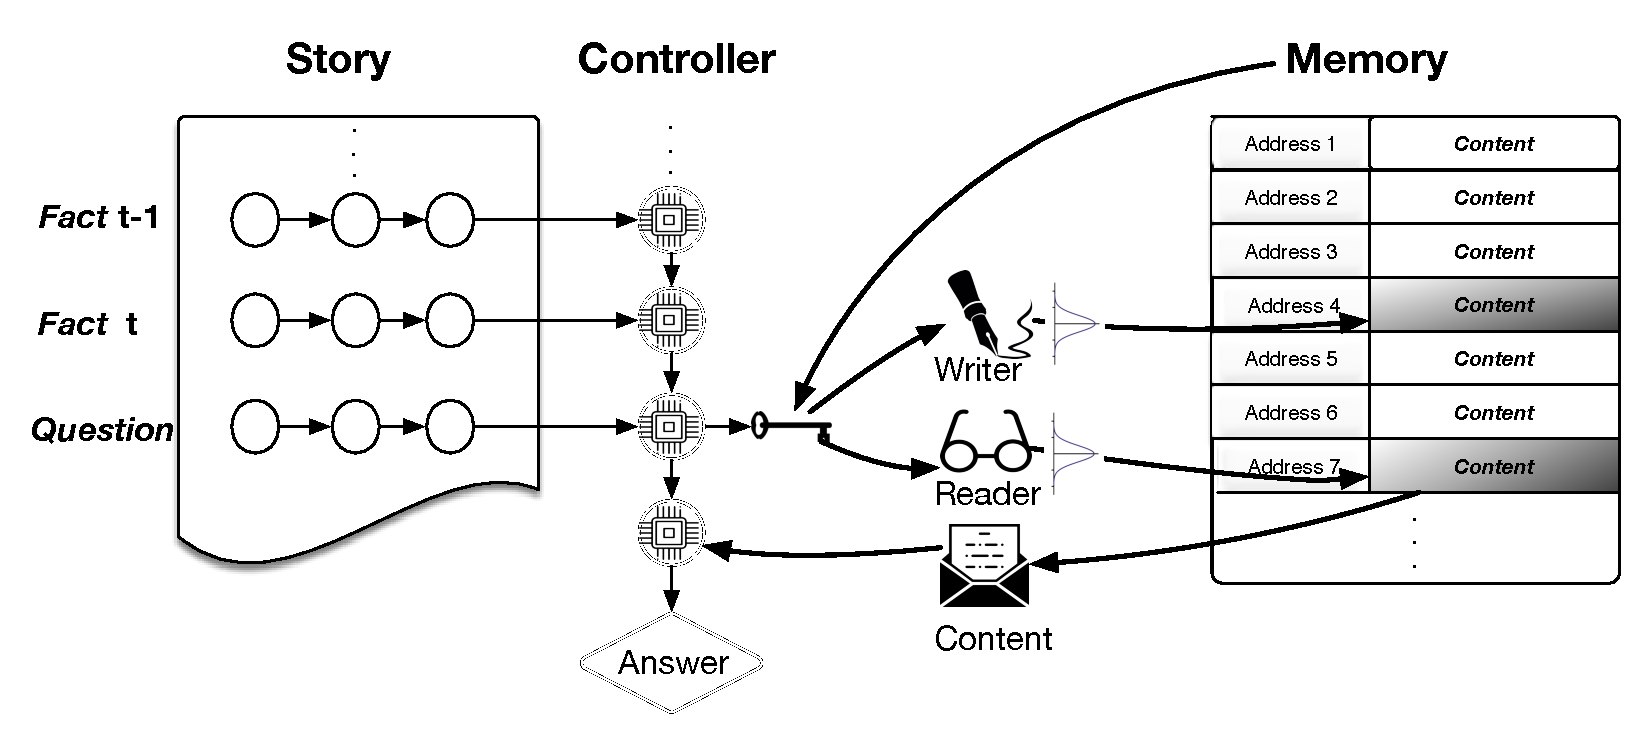
\includegraphics[width=0.94\textwidth]{NTM_QA_Overview_last}
\end{minipage}
A graphical illustration of the proposed dynamic neural Turing machine with the 
    recurrent-controller.  

\paragraph{Memory}
\[
    \mM = \left[ \mA ; \mC \right], ~
    \vm_i = \left[ \va_i ; \vc_i \right].
\]

\paragraph{No Operation (NOP)}

\paragraph{Multi-step Addressing}


\paragraph{Dynamic Least Recently Used Addressing}

\[
       \gamma_t = \text{sigmoid}(\vu_{\gamma} \vh_t + \vb_{\gamma}),~
       \vw_t \leftarrow \text{softmax}(\vz_t - \gamma_t \vv_{t-1}).
\]

\paragraph{Read-Write Consistency Regularizer}
\begin{align*}
    R_{\text{rw}}(\vw, \vu) = \lambda \sum_{t'=1}^{T}||1 -
    (\frac{1}{t'}\sum_{t=1}^{t'}\vu_t)^{\top}\vw_{t'} ||_2^2
\end{align*}
\paragraph{Discrete Addressing} 

\[
    p(j) = w_j,
\]
\[
    \tilde{w}_k = I(k=j),
\]

\paragraph{Training}
We use REINFORCE with input based baseline, 
\[
\tilde{R}(\vx) = \frac{R(\vx) - b}{\sqrt{\sigma^2 + \epsilon}},
\]
\[
\tilde{R}(\vx) \leftarrow \tilde{R}(\vx) - b(\vx),
\]

}
\headerbox{Experiments}{name=experiments,column=2,row=0}{

~\\ {\bf GRU Controller \\}

\scalebox{0.56}{
\begin{minipage}[t]{0.94\linewidth}
\vspace{-2mm}
  \centering
\small
\begin{tabular}{ | l || c | c | c || c |c |c|c|| c | c | c|c| }
\hline
& & & & 1-step & 1-step & 1-step & 1-step & 3-steps & 3-steps & 3-steps & 3-steps\\ 
& & & & LBA & CBA & Soft & Discrete & LBA & CBA & Soft & Discrete \\
Task & LSTM & MemN2N & DMN+ & NTM & NTM & D-NTM & D-NTM  & NTM & NTM & D-NTM & D-NTM\\ \hline
1 & 0.00 & 0.00 & 0.00 & 16.30 & 16.88 & 5.41 & 6.66 & 0.00 & 0.00 & 0.00 & 0.00\\
2 & 81.90 & 0.30 & 0.30 & 57.08 & 55.70 & 58.54 & 56.04 & 61.67 & 59.38 & 46.66 & 62.29\\
3 & 83.10 & 2.10 & 1.10 & 74.16 & 55.00 & 74.58 & 72.08 & 83.54 & 65.21 & 47.08 & 41.45\\
4 & 0.20 & 0.00 & 0.00 & 0.00 & 0.00 & 0.00 & 0.00 & 0.00 & 0.00 & 0.00 & 0.00\\
5 & 1.20 & 0.80 & 0.50 & 1.46 & 20.41 & 1.66 & 1.04 & 0.83 & 1.46 & 1.25 & 1.45\\
6 & 51.80 & 0.10 & 0.00 & 23.33 & 21.04 & 40.20 & 44.79 & 48.13 & 54.80 & 20.62 & 11.04\\
7 & 24.90 & 2.00 & 2.40 & 21.67 & 21.67 & 19.16 & 19.58 & 7.92 & 37.70 & 7.29 & 5.62\\
8 & 34.10 & 0.90 & 0.00 & 25.76 & 21.05 & 12.58 & 18.46 & 25.38 & 8.82 & 11.02 & 0.74\\
9 & 20.20 & 0.30 & 0.00 & 24.79 & 24.17 & 36.66 & 34.37 & 37.80 & 0.00 & 39.37 & 32.50\\
10 & 30.10 & 0.00 & 0.00 & 41.46 & 33.13 & 52.29 & 50.83 & 56.25 & 23.75 & 20.00 & 20.83\\
11 & 10.30 & 0.10 & 0.00 & 18.96 & 31.88 & 31.45 & 4.16 & 3.96 & 0.28 & 30.62 & 16.87\\
12 & 23.40 & 0.00 & 0.00 & 25.83 & 30.00 & 7.70 & 6.66 & 28.75 & 23.75 & 5.41 & 4.58\\
13 & 6.10 & 0.00 & 0.00 & 6.67 & 5.63 & 5.62 & 2.29 & 5.83 & 83.13 & 7.91 & 5.00\\
14 & 81.00 & 0.10 & 0.20 & 58.54 & 59.17 & 60.00 & 63.75 & 61.88 & 57.71 & 58.12 & 60.20\\
15 & 78.70 & 0.00 & 0.00 & 36.46 & 42.30 & 36.87 & 39.27 & 35.62 & 21.88 & 36.04 & 40.26\\
16 & 51.90 & 51.80 & 45.30 & 71.15 & 71.15 & 49.16 & 51.35 & 46.15 & 50.00 & 46.04 & 45.41\\
17 & 50.10 & 18.60 & 4.20 & 43.75 & 43.75 & 17.91 & 16.04 & 43.75 & 56.25 & 21.25 & 9.16\\
18 & 6.80 & 5.30 & 2.10 & 3.96 & 47.50 & 3.95 & 3.54 & 47.50 & 47.50 & 6.87 & 1.66\\
19 & 90.30 & 2.30 & 0.00 & 75.89 & 71.51 & 73.74 & 64.63 & 61.56 & 63.65 & 75.88 & 76.66\\
20 & 2.10 & 0.00 & 0.00 & 1.25 & 0.00 & 2.70 & 3.12 & 0.40 & 0.00 & 3.33 & 0.00\\\hline
Avg.Err. & 36.41 & 4.24 & \textbf{2.81} & 31.42 & 33.60 & 29.51 & \textbf{27.93} & 32.85 & 32.76 & 24.24 & \textbf{21.79}\\\hline
\end{tabular}
\end{minipage}}

~\\ {\bf Feedforward Controller \\}

\scalebox{0.7}{
\begin{minipage}[t]{0.95\linewidth}
\vspace{-2mm}
  \centering
  %\small 
\begin{tabular}{| l || c | c | c || c |c |c|}
\hline
& & & & Soft & Discrete & Discrete$^\ast$  \\
Task & LSTM & MemN2N & DMN+ & D-NTM & D-NTM  & D-NTM \\ \hline
1 & 0.00 & 0.00 & 0.00 & 4.38 & 81.67 & 14.79 \\
2 & 81.90 & 0.30 & 0.30 & 27.5 & 76.67 & 76.67 \\
3 & 83.10 & 2.10 & 1.10 & 71.25 & 79.38 & 70.83 \\
4 & 0.20 & 0.00 & 0.00 & 0.00 & 78.65 & 44.06 \\
5 & 1.20 & 0.80 & 0.50 & 1.67 & 83.13 & 17.71 \\
6 & 51.80 & 0.10 & 0.00 & 1.46 & 48.76 & 48.13 \\
7 & 24.90 & 2.00 & 2.40 & 6.04 & 54.79 & 23.54 \\
8 & 34.10 & 0.90 & 0.00 & 1.70 & 69.75 & 35.62 \\
9 & 20.20 & 0.30 & 0.00 & 0.63 & 39.17 & 14.38 \\
10 & 30.10 & 0.00 & 0.00 & 19.80 & 56.25 & 56.25 \\
11 & 10.30 & 0.10 & 0.00 & 0.00 & 78.96 & 39.58 \\
12 & 23.40 & 0.00 & 0.00 & 6.25 & 82.5 & 32.08 \\
13 & 6.10 & 0.00 & 0.00 & 7.5 & 75.0 & 18.54 \\
14 & 81.00 & 0.10 & 0.20 & 17.5 & 78.75 & 24.79 \\
15 & 78.70 & 0.00 & 0.00 & 0.0 & 71.42 & 39.73 \\
16 & 51.90 & 51.80 & 45.30 & 49.65 & 71.46 & 71.15\\
17 & 50.10 & 18.60 & 4.20 & 1.25 & 43.75 & 43.75 \\
18 & 6.80 & 5.30 & 2.10 & 0.24 & 48.13 & 2.92 \\
19 & 90.30 & 2.30 & 0.00 & 39.47 & 71.46 & 71.56\\
20 & 2.10 & 0.00 & 0.00 & 0.0 & 76.56 & 9.79 \\\hline
Avg.Err. & 36.41 & 4.24 & \textbf{2.81} & \textbf{12.81} & 68.30 & 37.79\\\hline
\end{tabular}
\end{minipage}}

\begin{minipage}[t]{0.95\linewidth}
\centering
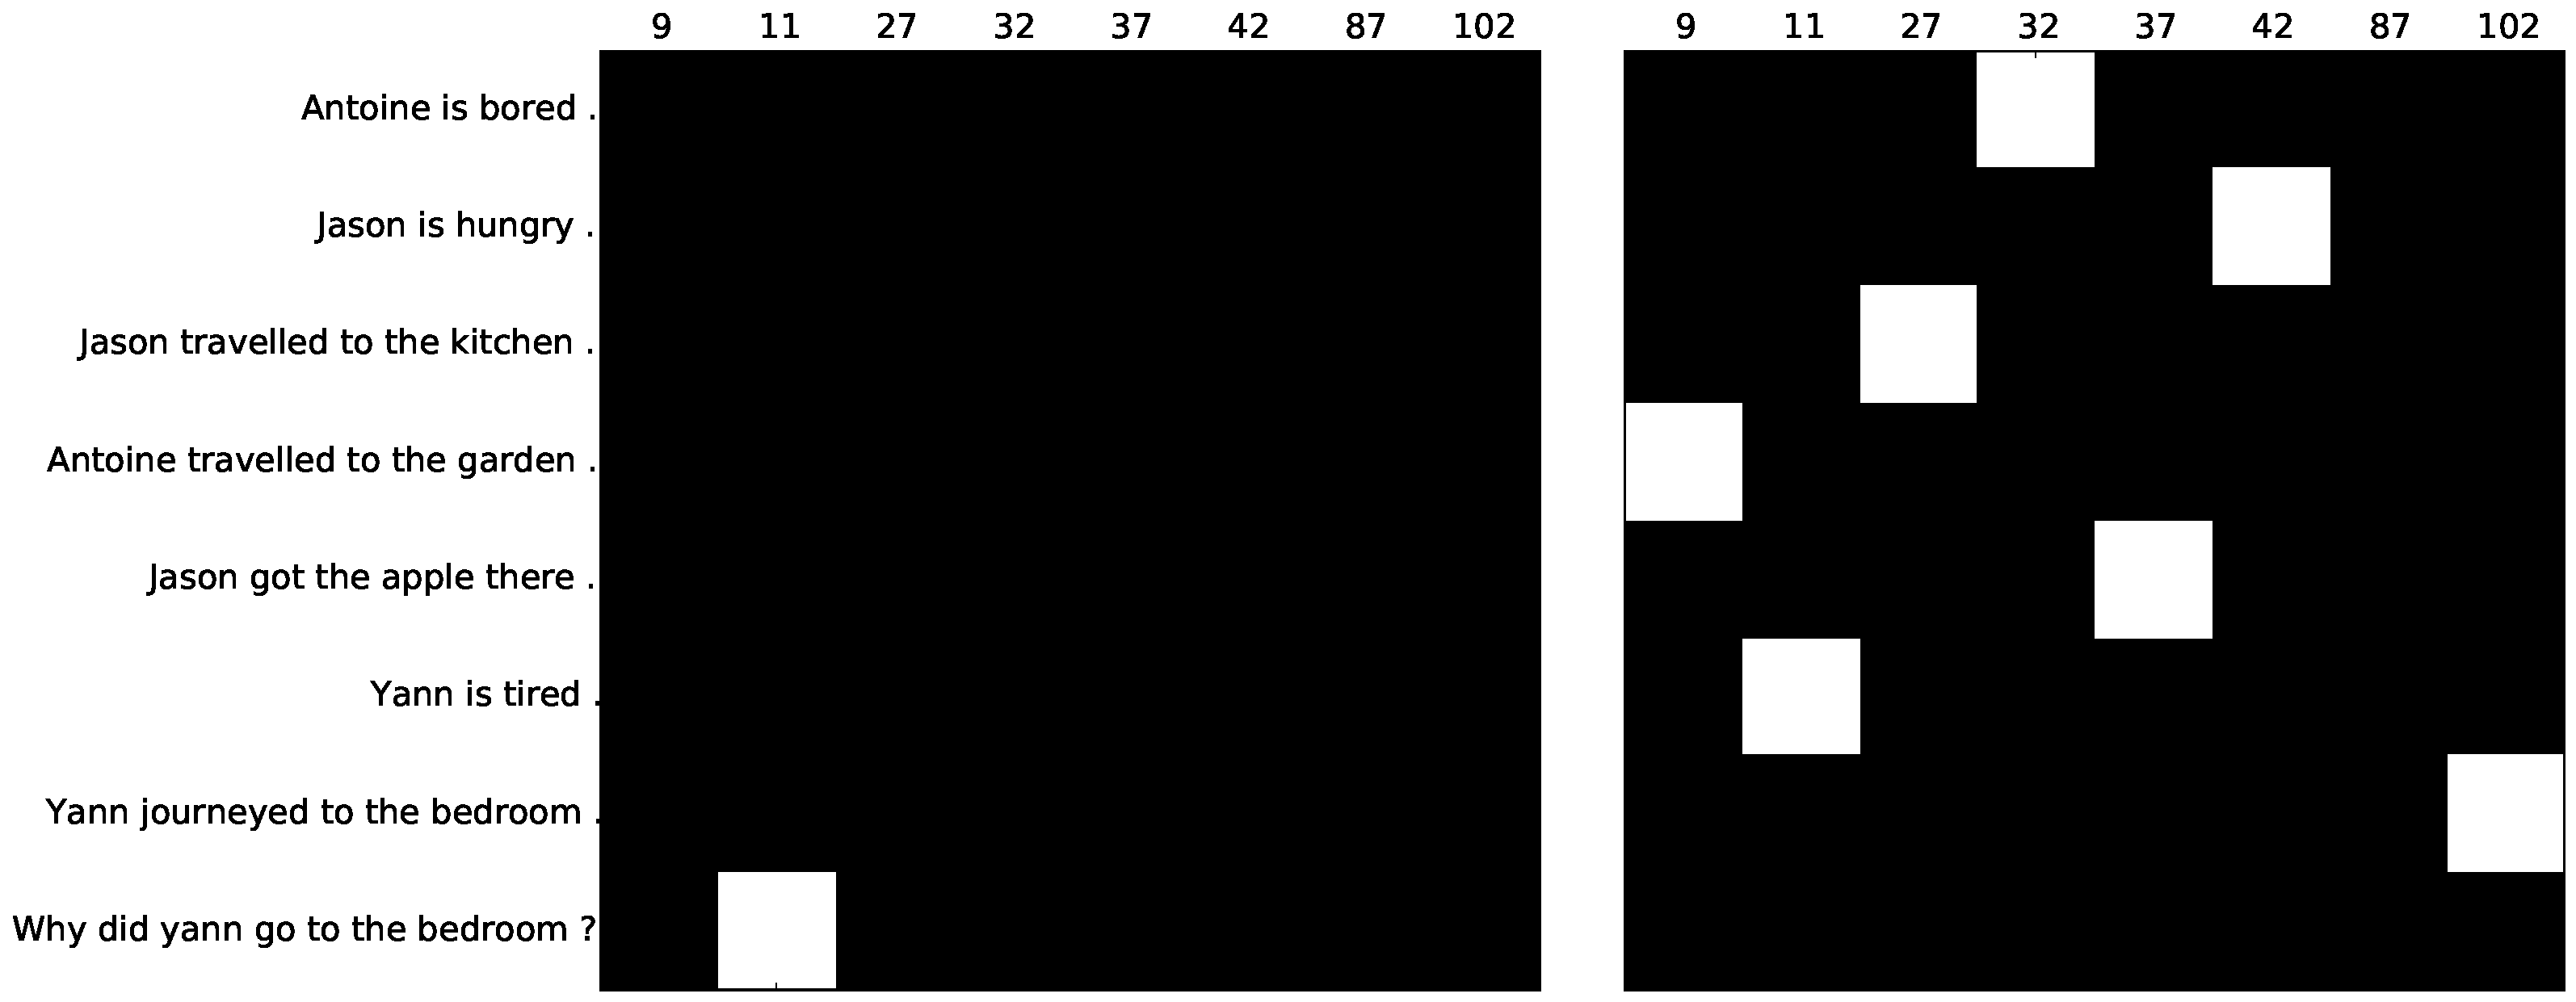
\includegraphics[width=0.94\textwidth]{ntm_grucontroller_task20_ntm_ex5_hard}
\end{minipage}
}
%}
%----------------------------------------------------------------------------------------
%	FUTURE RESEARCH
%----------------------------------------------------------------------------------------

%----------------------------------------------------------------------------------------
%	CONTACT INFORMATION
%----------------------------------------------------------------------------------------

%----------------------------------------------------------------------------------------
%	CONCLUSION
%----------------------------------------------------------------------------------------
%----------------------------------------------------------------------------------------
%	MATERIALS AND METHODS
%----------------------------------------------------------------------------------------

%----------------------------------------------------------------------------------------
%	RESULTS 2
%----------------------------------------------------------------------------------------

%----------------------------------------------------------------------------------------

\end{poster}

\end{document}
